\documentclass[preprint, review, authoryear, longtitle, 12pt, 3p]{elsarticle}
\usepackage{booktabs}
\usepackage{makecell}
\usepackage{amsmath}
\usepackage{amssymb}
\usepackage{graphicx}
\usepackage[labelfont=bf, justification=raggedright, singlelinecheck=false]{caption}
\usepackage{hyperref}
\usepackage{lineno}
\usepackage{setspace}

\doublespacing
\captionsetup[figure]{name=Fig. ,labelsep=period}
\captionsetup[table]{name=Table ,labelsep=period}
\graphicspath{{./fig/}}

\begin{document}

\begin{frontmatter}
  \title{Intercomparison of runoff and river discharge reanalysis datasets: Insights from the Upper Jinsha River, an alpine river at the eastern edge of the Tibetan Plateau}

  \author[1]{Shuanglong Chen\fnref{fn1}}
  \ead{chen_shuanglong@ctg.com.cn}

  \author[2]{Heng Yang\fnref{fn1}}
  \ead{yang_heng2@ctg.com.cn}

  \author[3]{Hui Zheng\corref{cor1}}
  \ead{hzheng\_iap@outlook.com}

  \fntext[fn1]{These authors contributed equally to this work and should be considered co-first authors.}

  \cortext[cor1]{Corresponding author}

  \affiliation[1]{organization={Baihetan Hydropower Plant, China Three Gorges Corporation}, postcode={615421}, city={Sichuan}, country={China}}
  \affiliation[2]{organization={Science and Technology Research Institute, China Three Gorges Corporation}, postcode={100038}, city={Beijing}, country={China}}
  \affiliation[3]{organization={Institute of Atmospheric Physics, Chinese Academy of Sciences}, postcode={100029}, city={Beijing}, country={China}}

  \begin{abstract}
    The availability of runoff and river discharge reanalysis datasets is rapidly increasing. These datasets use different meteorological forcing, land surface models, river routing methods, river networks, calibration data, and calibration methods. This diversity calls for intercomparison. This study intercompares ERA5-Land, GloFAS, GRFR, and CNRD in the Upper Jinsha River, an alpine river on the eastern edge of the Tibetan Plateau. We include a high-resolution runoff simulation using the NoahMP land surface model and ERA5-Land meteorological data in the intercomparison to assess the influence of meteorological inputs, spatial resolution, and calibration on runoff estimation. The runoff from these datasets is rerouted on a high-resolution river network delineated from the 3-arcsecond MERIT-Hydro dataset, enabling us to evaluate the effects of routing models and river network delineations on discharge estimates. Our analysis is based on observations at three gauging stations—Zhimenda, Gangtuo, and Benzilan—at monthly, daily, and hourly scales. Results indicate that the calibration of land surface or hydrological models significantly impacts runoff and river discharge estimates, potentially more than meteorological data. Calibrated datasets, GloFAS and GRFR, outperform the others, despite being driven by different forcings. The runoff characteristics-based calibration method, as seen in GRFR, yields superior performance, with rerouted hourly river discharge using GRFR runoff achieving a high Kling-Gupta Efficiency of approximately 0.9. Accurate river network delineation with high-resolution hydrography data is crucial. The high performance of GloFAS discharge, contrasting with its runoff, is likely attributed to the coarse routing grid resolution. These insights can guide further improvements in the reanalyses.
  \end{abstract}

  \begin{highlights}
  \item The calibration of land surface models exerts a significant influence on the accuracy of runoff and river discharge estimations
  \item The runoff characteristics-based calibration method is highly effective for runoff estimation
  \item High-resolution simulations can yield distinct runoff characteristics compared to their low-resolution counterparts
  \item High-resolution river network delineation is essential for the concurrent enhancement of runoff and discharge estimations
  \item Intercomparison can identify deficiencies within model configurations and inform subsequent refinements
  \end{highlights}

  \begin{keyword}
    river discharge \sep runoff \sep model intercomparison \sep the upper Jinsha River
  \end{keyword}
\end{frontmatter}

\section{Introduction}

The proliferation of global- and continental-scale runoff and discharge reanalysis datasets has been a significant development in hydrological research. Datasets such as the European Centre for Medium-Range Weather Forecasts (ECMWF) Reanalysis version 5 (ERA5) \citep{hersbach2020QJMRS}, ERA5-Land \citep{munoz-sabater2021ESSD}, the Global Flood Awareness System (GloFAS) \citep{alfieri2020JH, harrigan2020ESSD}, and the Global Reach-Level Flood Reanalysis (GRFR) \citep{yang2021BAMS, lin2019WRR} offer continuous and spatially comprehensive estimates of runoff and river discharge on a global scale. Additionally, regional datasets like the National Water Model (NWM) of the United States \citep{cosgrove2024JAWRA}, the European Flood Early Warning Systems \citep{najafi2024NC}, and the China Natural Runoff Dataset (CNRD) \citep{gou2021BAMS, miao2022CSB} provide runoff and discharge estimates tailored to specific regions. These datasets have significantly advanced our scientific understanding of river systems \citep{feng2021NC, collins2024NG} and their complex interactions with other components of the Earth system \citep{liu2024NG}. Furthermore, they have been instrumental in supporting decision-making processes, particularly in the area of water-resources utilization and flood protection \citep{cosgrove2024JAWRA, coughlan_de_perez2016HESS}.

These reanalysis datasets of runoff and river discharge are generated through a complex chain of methodologies that include meteorological forcing data, land surface models or hydrological models, river routing models, river network delineations, and calibrations. The diversity within these components can significantly influence the estimation of runoff and river discharge. Studies have demonstrated that meteorological forcing data can differ remarkably \citep{sun2018RG, henn2018JH}. The use of different meteorological forcing data \citep{renard2010WRR, bai2024JGRA}, in combination with varying model structure \citep{butts2004JH}, spatial resolutions \citep{haddeland2002WRR, barnhart2024WRR, li2022GMD}, parameterizations \citep{zheng2019WRR,zheng2023ESSD}, and parameters \citep{li2020JAMS} of land surface models or hydrological models, can lead to disparate estimates of runoff \citep{saxe2021HESS, beck2017HESS}. Furthermore, these differences in runoff estimation can be further amplified by the methods employed in river routing \citep{fry2014JH, mai2022HESS, ahmed2023JH}.

The diversity presented in the estimation methodologies call for careful intercomparison before the use of reanalysis datasets. In the past decades, a variety of intercomparison studies have been conducted with different objectives. Land surface model comparisons such as the Project for Intercomparison of Land-surface Parameterization Schemes \citep{henderson-sellers1993BAMS} and the Land Surface, Snow and Soil Moisture Model Intercomparison Project \citep{van_den_hurk2016GMD} conducted with the same meteorological forcing data greatly help to reveal the weakness of the participant models and the interactions of land surface processes. The Distributed Model Intercomparison Project \citep{reed2004JH, smith2004JH} compared distributed models with lumped models. This project revealed the superiority of distributed routing models in reproducing flood peaks and reported the importance of calibration on distributed rainfall-runoff models. \citet{beck2017HESS} compares ten hydrological models at the global scale. Their results further confirm the importance of calibration of model parameters in accurate runoff estimation. The Continental Hydrological Intercomparison Project \citep{tijerina2021WRR} compares two high-resolution, physics-based models at the continental scale. The intercomparison promotes high-resolution modeling to enhance topographic processing and to improve topographic representation over complex topography. There are also intercomparisons with regional focuses. The Great Lakes Runoff Intercomparison Project \citep{mai2022HESS} and the Nelson Model Intercomparison Project under the Integrated Modelling Program of Canada initiative \citep{ahmed2023JH} are two examples. These intercomparison studies aim to select the best-performing estimation methodologies for the region and guide further improvements of operations.

The Upper Jinsha River, serving as the source of the Changjiang River, is notable for its pronounced vertical drop and substantial hydroelectric potential. The river is located on the eastern edge of the Tibetan Plateau. To date, thirteen hydroelectric facilities have been constructed or are in the planning stages along the main stem of the Upper Jinsha River, collectively possessing an installed capacity of approximately 14.6 gigawatts. The river originates from the Tibetan Plateau. The source area of the river consists of a major part of the Sanjiangyuan National Nature Reserve, the highest and largest nature reserve in China yet. The operations of the hydroelectric facilities and the natural reserves demand accurate estimation of water resources. However, hydrometeorological observations are scarce in the region. The complex topography, the high-alpine environment, and the strong demand for accurate runoff and river discharge estimates make the Upper Jinsha River an ideal testbed for runoff and river discharge reanalysis datasets.

This study is designed to intercompare runoff and river discharge reanalysis data obtained from ERA5-Land, GloFAS, GRFR, and CNRD. As a pilot effort of such reanalysis intercomparisons, this study focuses specifically on the Upper Jinsha River. The primary objective is to assess the effectiveness and identify any shortcomings of the methodologies employed in these reanalyses. The findings from this intercomparison are expected to provide valuable insights that will guide future enhancements in the estimation of runoff and river discharge within the region.

\section{Data and methods}

\subsection{Study area and river network delineation}

Figure~\ref{fig:domain} illustrates the terrain and river network of the upper Jinsha River. The study area encompasses the region upstream of the Benzilan gauging station. The elevation within the study area ranges from approximately 6600~m at its highest point to approximately 2000~m at its lowest. The river network was extracted from the Multi-Error-Removed Improved-Terrain Hydrography (MERIT-Hydro) dataset~\citep{yamazaki2019WRR, yamazaki2017GRL}. MERIT-Hydro is a globally recognized dataset providing hydrologically conditioned elevation, flow direction, and flow accumulation area data, with a spatial resolution of 3 arc-seconds. The extraction of the river network was based on the flow accumulation area, using a threshold of 25~km\textsuperscript{2}, which resulted in the identification of 5,787 river reaches within the study area.

\begin{figure}[ht!]
  \centering
  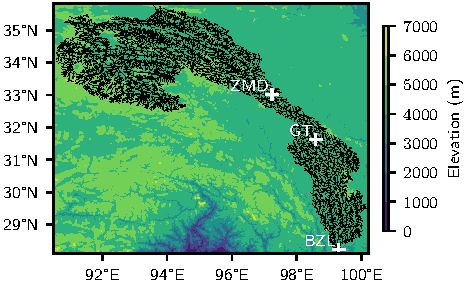
\includegraphics[width=0.8\textwidth]{domain.pdf}
  \caption{The study domain and river network of the source region of the upper Jinsha River. The white crosses indicate the location of the gauging stations: ZMD for Zhimenda, GT for Gangtuo, BT for Batang, and BZL for Benzilan.}
  \label{fig:domain}
\end{figure}

\subsection{Reanalysis Datasets}

Table~\ref{tab:dataset} presents an overview of the datasets employed in this study. ERA5-Land~\citep{munoz-sabater2021ESSD} is an enhanced global dataset, an improvement over ERA5~\citep{hersbach2020QJMRS}. This dataset features a substantial enhancement in spatial resolution, with an increase from ERA5's 31 km to 0.1\textdegree{} globally. A variety of land surface variables, including runoff, are simulated using the Carbon Hydrology-Tiled ECMWF Scheme for Surface Exchanges over Land (CHTESSEL) model~\citep{boussetta2021A, balsamo2009JHM}, operating at an hourly temporal resolution.

The GloFAS historical reanalysis version 4.0~\citep{alfieri2020JH, harrigan2020ESSD} is another dataset produced by the European Centre for Medium-Range Weather Forecasts (ECMWF), with a focus on hydrological variables. GloFAS shares the same spatial resolution of 0.1\textdegree{} as ERA5-Land. It is driven by ERA5 meteorological data, which is highly similar to ERA5-Land. The primary distinctions between GloFAS and ERA5-Land lie in the hydrological model employed, the temporal resolution, and the output variables. GloFAS utilizes the LISFLOOD model~\citep{knijff2010IJGIS} at a daily time step. Unlike ERA5-Land, the parameters of LISFLOOD are calibrated against daily river discharge observations using an evolutionary algorithm~\citep{hirpa2018JH}. LISFLOOD simulates both runoff and river discharge, whereas ERA5-Land provides only runoff estimates.

The GRFR dataset~\citep{yang2021BAMS} is a comprehensive global dataset providing runoff and river discharge data at a 3-hourly temporal resolution. The runoff is simulated using the Variable Infiltration Capacity (VIC) model~\citep{liang1994JGRA} at a spatial resolution of 0.05\textdegree, which is driven by precipitation data from the Multi-Source Weighted-Ensemble Precipitation (MSWEP) dataset~\citep{beck2019BAMS} and other meteorological variables from ERA5. The VIC model's parameters are calibrated~\citep{yang2019WRR} at each 0.05\textdegree{} grid cell against a machine-learning-derived runoff characteristics dataset produced by~\citet{beck2015JHM}. The bias in the VIC-simulated runoff is further corrected using the same runoff characteristics dataset, following the methodology of~\citet{lin2019WRR}. The calibrated and bias-corrected runoff data are then utilized to drive the Routing Application for Parallel computatIon of Discharge (RAPID) river routing model~\citep{david2011JHM} for simulating river discharge. The parameters of RAPID are estimated using a statistical relationship that correlates discharge with river width, water depth, channel slope, and celerity~\citep{lin2019WRR}. The river network employed in the routing process is also derived from the MERIT Hydro dataset~\citep{lin2021SD}.

The China Natural Runoff Dataset (CNRD) \citep{gou2021BAMS, miao2022CSB} comprises runoff data at a 0.25° spatial resolution. This dataset is simulated using the VIC model, driven by the China Meteorological Forcing Dataset \citep{he2020SD}. The parameters of the VIC model were calibrated against river discharge observations from approximately 200 catchments across China and then extrapolated to ungauged river basins using the multiscale regionalization method \citep{samaniego2010WRR}.

The quality of runoff and river discharge reanalyses is influenced by various factors, including meteorological forcing, land surface model/hydrological model, river network routing model, model resolution, and parameter settings. In this study, we produced a new dataset for comparison. As detailed in Table~\ref{tab:dataset}, our dataset boasts the highest spatial and temporal resolution, employs an advanced land surface model, and utilizes the most sophisticated river routing method among the datasets examined. The dataset is generated using the Noah with Multi-Parameterization (NoahMP) land surface model \citep{niu2011JGRA}, which is driven by ERA5-Land meteorological data. The static parameters for NoahMP are derived from the Weather Research and Forecasting geographic static data (\url{https://www2.mmm.ucar.edu/wrf/users/download/get_sources_wps_geog.html}). NoahMP operates at a spatial resolution of 0.01° from 2008 to 2016. The initial condition for 2008 is sourced from ERA5-Land. The first year is allocated for model spin-up, with the simulated runoff from 2009 to 2016 used for analysis. NoahMP offers a variety of parameterization schemes for land surface processes, and we adopted the same schemes as those used in the NWM of the United States \citep{cosgrove2024JAWRA}. The runoff is routed using the variable-parameter Muskingum--Cunge (MC) method on the river network depicted in Figure~\ref{fig:domain} to estimate river discharge. The routing algorithm mirrors that of the NWM, assuming a trapezoidal channel cross-section. Channel cross-section geometry and roughness parameters are sourced from the default parameter lookup table of the NWM \citep{read2023JAWRA} and the Strahler stream order for each river reach within the network. In theory, the MC routing method would outperform the kinematic wave routing method used in GloFAS by also additionally considering diffusive wave dynamics, while the Muskingum routing method used in GRFR would be the least performing among the three. It is important to note that this comparison is theoretical, and actual performance can vary significantly with model implementation and parameter settings

\subsection{River discharge observations}\label{sec:obs}

We utilized river discharge observations from three gauging stations along the mainstream of the upper Jinsha River: Zhimenda (ZMD), Gangtuo (GT), and Benzilan (BZL), covering the period from 2009 to 2016. The selection of this timeframe is justified by the minimal presence of hydroelectric facilities, which ensures that the river discharge data are largely unaffected by human interventions.

The dataset from Zhimenda is compiled at a daily resolution. The dataset comprises 1,477 records, with 49\% of the days within the 2009 to 2016 period missing. In contrast, Gangtuo and Benzilan provide data at an hourly resolution, aaccumulating 52,246 hours and 69,011 hours, respectively. The respective missing data rates for these stations are 25\% for Gangtuo and 1.6\% for Benzilan. Given the nature of our analysis, we have chosen not to impute the missing values, opting instead to focus solely on the complete data records. This decision was made to preserve the integrity of the dataset and to mitigate the potential biases that could be introduced by gap-filling methods.

To our knowledge, the daily river discharge observations at Zhimenda have been used to calibrate GloFAS and GRFR, while the observations at Gangtuo and Benzilan have not been incorporated into the datasets analyzed in this study.

\begin{table}[ht!]
  \renewcommand{\arraystretch}{1.15}
  \caption{The datasets used in this study.}
  \label{tab:dataset}
  \centering
  \small
  \begin{tabular}{cccccc}
    \toprule
    Dataset & Time period & \thead{Temporal \\ Resolution} &
    \thead{Runoff \\ Resolution} & \thead{River \\ Routing} & References \\
    \midrule
    \multicolumn{6}{c}{\textit{Publically available datasets}} \\
    ERA5-Land & 1950--Present & Hourly & 0.10\textdegree & N/A & \citet{munoz-sabater2021ESSD} \\
    GloFAS v4.0 & 1979--Present & Daily & 0.10\textdegree & LISFLOOD & \citet{harrigan2020ESSD} \\
    GRFR v1.0 & 1980--2019 & 3-hourly & 0.05\textdegree & RAPID & \citet{yang2021BAMS} \\
    CNRD v1.0 & 1961--2018 & Monthly & 0.25\textdegree & N/A & \citet{miao2022CSB} \\
    \multicolumn{6}{c}{\textit{Datasets produced in this study}} \\
    \makecell{ERA5-Land/ \\ NoahMP} & 2009--2016 & Hourly & 0.01\textdegree & MC & This study\\
    \bottomrule
  \end{tabular}
\end{table}

\subsection{Evaluation methods}

As shown in Table~\ref{tab:dataset}, the datasets vary in spatial and temporal resolution. River discharge estimates are not available in every dataset examined. To address these inconsistencies, we remapped the runoff onto a common 0.01° grid and refined both daily and monthly values to hourly values, as depicted in Figure~\ref{fig:workflow}. The spatial remapping was conducted using a first-order conservative method. For temporal refinement, we used the fraction of hourly ERA5-Land runoff to the accumulated runoff within a day or a month to redistribute the daily or monthly values. Subsequently, the runoff from all datasets was routed using the same Muskingum--Cunge (MC) method, as previously described, to estimate river discharge. For GloFAS and GRFR, which provide river discharge estimates, we also refined the 3-hourly or daily values to hourly values using the same refinement method as the runoff.

The river discharge estimates derived from the Muskingum--Cunge method, as well as the temporally refined river discharge data from GRFR and GloFAS, are then compared with the observations at the gauging stations. This evaluation is conducted across three temporal scales—monthly, daily, and hourly—to comprehensively assess the accuracy and consistency of the estimates with the actual observations.

The structure and parameters of the river routing model significantly influence the river discharge estimates. To isolate the impact of river routing on these estimates, we not only compared the model-derived river discharge with observations at gauging stations but also aggregated the runoff above these stations for a more direct comparison. This aggregation helps to isolate the effects of routing by focusing on the input runoff rather than the routing process itself. The aggregated runoff is calculated by summing the runoff within the upstream area of each gauging station. The delineation of the upstream area was based on the flow direction data from the MERIT-Hydro dataset.

\begin{figure}[ht!]
  \centering
  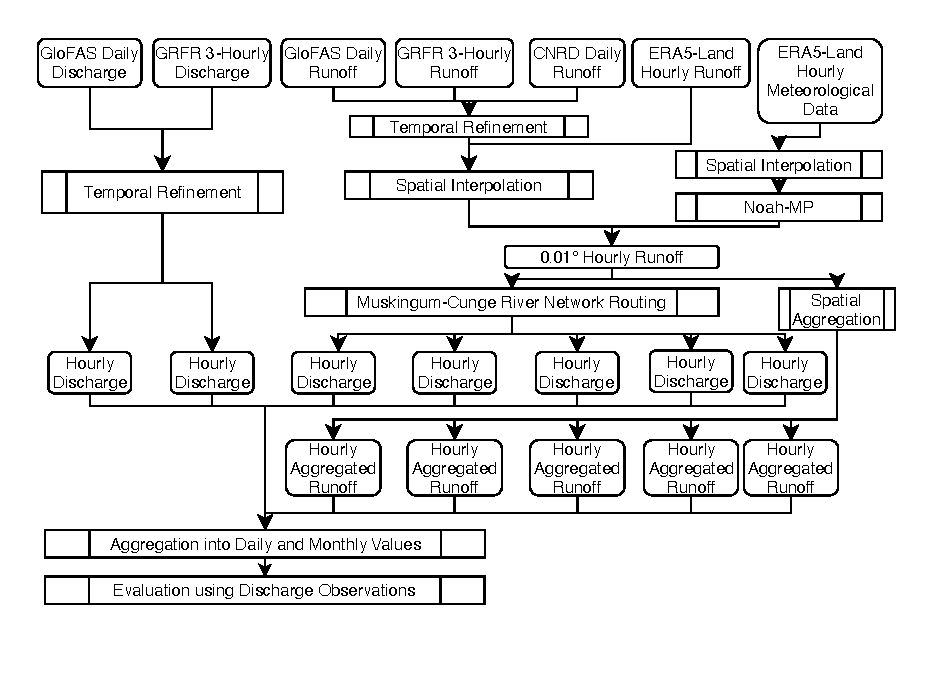
\includegraphics[width=\textwidth]{workflow.pdf}
  \caption{Workflow of this study.}
  \label{fig:workflow}
\end{figure}

\subsection{Evaluation metrics}

We employed the Kling-Gupta Efficiency (KGE) \citep{gupta2009JH} to assess the performance of the reanalysis datasets. The KGE is a comprehensive metric that encapsulates the correlation coefficient, the ratio of the standard deviations, and the ratio of the mean values of both observed and simulated data. The KGE is formulated as follows:
\begin{align}
  \label{eq:kge}
  \text{KGE} =& 1 - \sqrt{G_1^2 + G_2^2 + G_3^2} \text{,} \\
  G_1 =& r - 1 \text{,} \\
  G_2 =& \frac{\sigma_s}{\sigma_o} - 1 \text{,} \\
  G_3 =& \frac{\mu_s}{\mu_o} - 1 \text{,}
\end{align}
where $r$ is the correlation coefficient, $\sigma_s$ and $\sigma_o$ are the standard deviations of the simulated and observed data, respectively, and $\mu_s$ and $\mu_o$ are the mean values of the simulated and observed data, respectively. The KGE ranges from $-\infty$ to 1, with a value of 1 indicating a perfect match between the simulated and observed data. A KGE value significantly less than 1 indicates a poor match.

The relative contribution of the three terms in the KGE can be calculated using the following formula \citep{gupta2009JH}:
\begin{equation}
  g_i = \frac{G_i^2}{G_1^2 + G_2^2 + G_3^2} \text{,} \quad \text{for}
  \  i = 1, 2, 3 \text{,}
\end{equation}
where $g_1$, $g_2$, and $g_3$ are the relative contributions of correlation coefficient, variability, and bias, respectively. A higher value indicates a greater contribution of the corresponding term to the deviation of the KGE from 1.

\section{Results and discussion}

\subsection{Runoff}

Figure~\ref{fig:runoff_spatial} geographically compares the runoff estimates within the Benzilan catchment.The five examined datasets fall into three categories: the first includes ERA5-Land and ERA5-Land/NoahMP, the second includes GloFAS and GRFR, and the third includes CNRD. The first group utilizes uncalibrated land surface models, the second group employs extensively calibrated hydrological models, and the third group features a hydrological model with parameters that are regionalized rather than individually calibrated. It is intriguing to note that ERA5-Land, ERA5-Land/NoahMP, and GloFAS exhibit significant differences, despite their meteorological forcing data being similar. On the other hand, GloFAS and GRFR, which are driven by different meteorological forcing data, show close spatial patterns. This comparison indicates that the calibration of land surface models or hydrological models has a profound impact on runoff estimation, more than the meteorological data.

\begin{figure}[ht!]
  \centering
  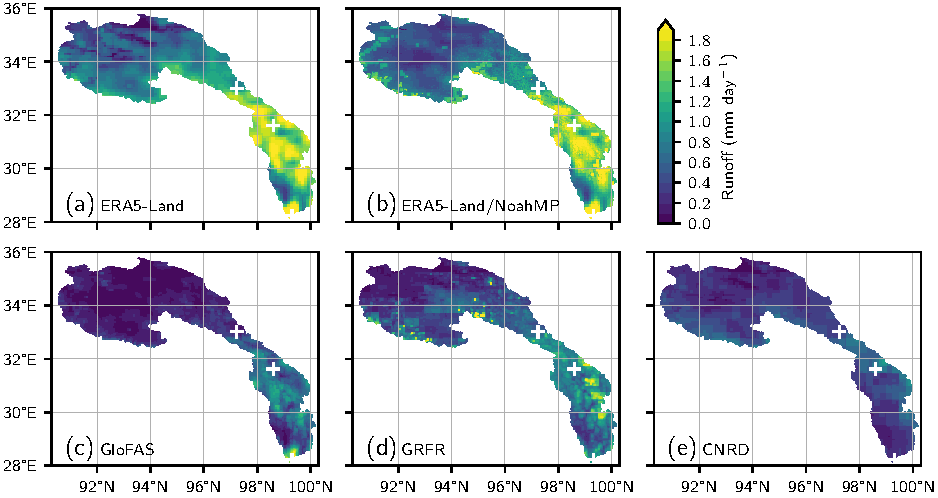
\includegraphics[width=\textwidth]{runoff_mean.pdf}
  \caption{Intercomparison of the spatial distribution of multiyear averaged runoff from 2009 to 2016.}
  \label{fig:runoff_spatial}
\end{figure}

Figure~\ref{fig:runoff_agg_ts} intercompares the monthly variations and annual cycle of the aggregated runoff above Zhimenda, Gangtuo, and Benzilan. Since the river flow travel time is typically smaller than a month \citep{allen2018GRL}, it is generally safe to neglect the impact of river routing at the monthly time scale. Both ERA5 and CNRD overestimate the runoff at all examined stations, but the reasons for this overestimation differ. The overestimation of ERA5 is consistent with previous studies, which link it to overestimated precipitation in high altitude regions \citep{bian2019JHM, bian2020JGRA, sun2021ERL, wang2024RS}. In contrast, the overestimation of CNRD is primarily observed in the upstream area of Zhimenda. Given that CMFD, the meteorological data that drive CNRD, has shown closeness to in-situ precipitation observations in this region \citep{wang2024RS}, the overestimation of the CNRD runoff is likely due to less constrained hydrological model parameters. CNRD uses parameters calibrated at gauged basins and extrapolates these parameters to ungauged basins using multiscale regionalization functions \citep{gou2021BAMS, miao2022CSB}. The scarcity of river discharge gauges on the Tibetan Plateau means that this extrapolation can lead to bias.

The runoff from ERA5-Land/NoahMP exhibits two peaks, particularly in the high-altitude regions above Zhimenda. In contrast, ERA5-Land, which utilizes the same meteorological data, shows an insignificant rise in runoff during Spring. The discrepancy between ERA5-Land/NoahMP and ERA5-Land would be attributed to the spatial resolution of the land surface model. The higher resolution of ERA5-Land/NoahMP allows for a better capture of the vertical gradient of land surface temperature. The combination of overestimated precipitation in the ERA5-Land meteorological data and increased snowmelt in low-altitude model grids \citep{barnhart2024WRR} results in a factitious Spring runoff peak that is not observed in actual data.

The two calibrated datasets, GloFAS and GRFR, exhibit distinct behaviors. This difference is even evident at Zhimenda, where observations are publicly available through the Global Runoff Data Centre and have been utilized in both datasets. The distinct calibration approaches of the two datasets likely account for this difference. GloFAS is calibrated against river discharge observations \citep{hirpa2018JH}, while its runoff is not directly calibrated. Since river discharge can be calculated by multiplying the catchment area by runoff, different estimates of the catchment area will lead to different runoff values after the calibration of river discharge. In contrast, GRFR's runoff is directly calibrated against a machine-learning-derived runoff characteristics dataset \citep{yang2019WRR}. The results suggest that the calibration method employed by GRFR is highly effective, yielding the best-performing runoff among the examined datasets.

\begin{figure}[ht!]
  \centering
  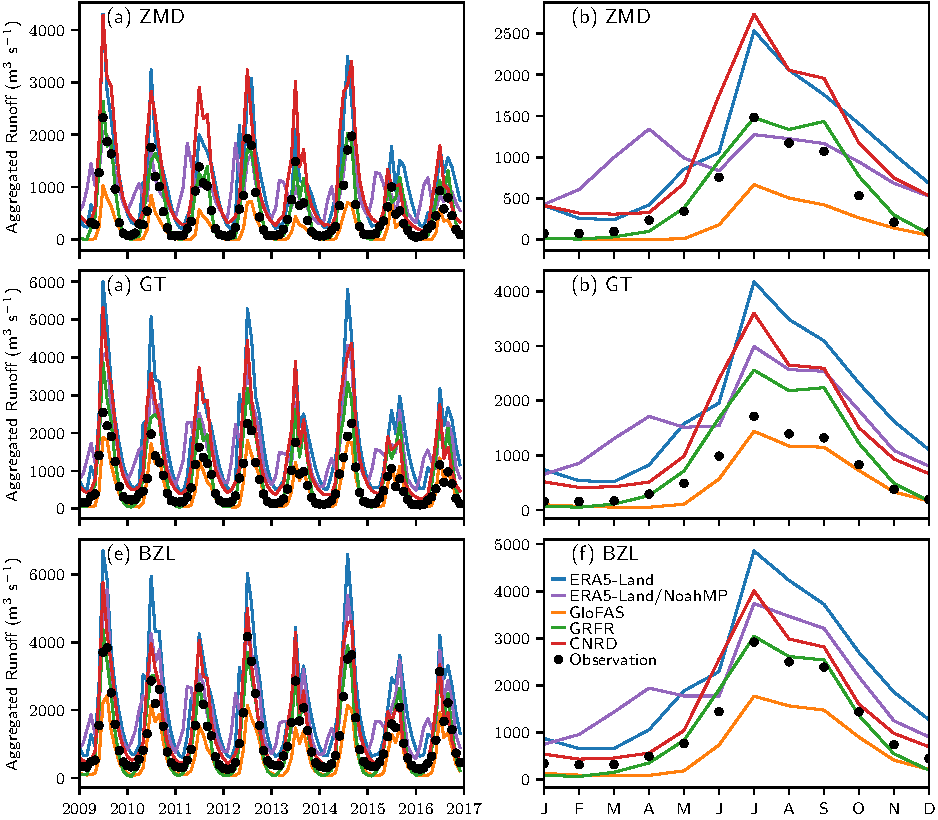
\includegraphics[width=\textwidth]{runoff_agg_ts.pdf}
  \caption{Intercomparison of the aggregated runoff at the gauging stations. (a) monthly aggregated runoff at Zhimenda; (b) annual cycle of the aggregated runoff at Zhimenda; (c) monthly aggregated runoff at Gangtuo; (d) annual cycle of the aggregated runoff at Gangtuo; (e) monthly aggregated runoff at Benzilan; and (f) annual cycle of the aggregated runoff at Benzilan.}
  \label{fig:runoff_agg_ts}
\end{figure}

Figure~\ref{fig:runoff_kge} presents the performance of the aggregated runoff in comparison with discharge observations at the monthly time scale. ERA5-Land consistently underperforms across all stations and time scales, corresponding to the overestimation shown in Figure~\ref{fig:runoff_agg_ts}. CNRD also performs poorly in high-altitude areas above Gangtuo due to overestimation, but its performance improves at Benzilan. The performance of CNRD slightly outperforms the high-resolution ERA5-Land/NoahMP. Among the examined datasets, the two calibrated datasets, GloFAS and GRFR, perform the best at almost every station examined, highlighting the importance of calibration for land surface models or hydrological models. Notably, GRFR's performance is exceptionally good, with a KGE above 0.8 at Zhimenda and Benzilan. The high performance of GRFR suggests the effectiveness of the characteristics-based calibration method.

\begin{figure}[ht!]
  \centering
  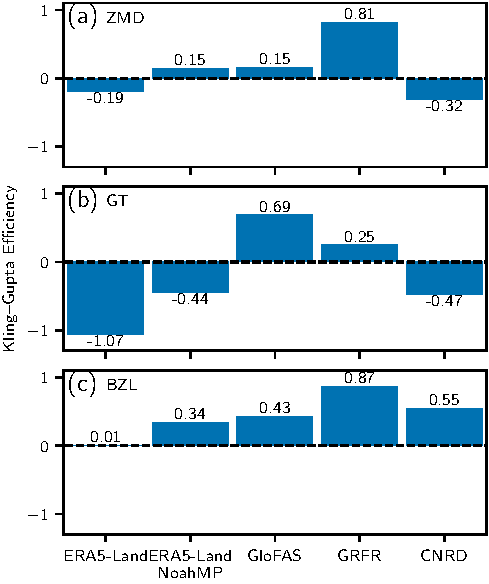
\includegraphics[width=0.5\textwidth]{runoff_agg_kge_mon.pdf}
  \caption{Kling--Gupta Efficiency of the monthly aggregated runoff. (a) the measures at Zhimenda, (b) the measures at Gangtuo, and (c) the measures at Benzilan.}
  \label{fig:runoff_kge}
\end{figure}

\subsection{Streamflow}

Figure~\ref{fig:streamflow_ts} compares the monthly discharge estimations with observations. The patterns generally follow the runoff pattern shown in Figure~\ref{fig:runoff_agg_ts}. The overestimation observed in ERA5-Land and CNRD closely mirrors their runoff overestimation. The artificial Spring peak, which is also present in the ERA5-Land/NoahMP discharge, aligns with the runoff pattern.

It is interesting to note that the GloFAS and GRFR discharge behave differently from the runoff. Our rerouted GloFAS runoff (GloFAS-MC in Figure~\ref{fig:streamflow_ts}) can reproduce the underestimated patterns observed for the runoff (Figure~\ref{fig:runoff_agg_ts}), confirming that GloFAS underestimates runoff. However, the underestimation of runoff is no longer presented in the river discharge. GloFAS closely reproduced the observed river discharge (Figure~\ref{fig:streamflow_ts}). The contradiction between the runoff underestimation and the unbiased discharge estimation suggests that the spatial resolution of GloFAS's routing grid plays a role. GloFAS is routed on a $\frac{1}{10}$° grid cell basis, whereas the river basins delineated in this study (as shown in Figure~\ref{fig:domain}) are based on $\frac{1}{1200}$° grids. The resolution of GloFAS may be too coarse to accurately delineate the river basins. However, this error is mitigated in the discharge due to the calibration, and the impact is transferred to errors in the runoff.

Despite the high skill of GRFR's runoff demonstrated in Figure~\ref{fig:runoff_agg_ts}, the skill of GRFR's discharge is unexpectedly unsatisfactory. GRFR remarkably overestimates discharge at all gauging stations. Meanwhile, our estimated discharge (GRFR-MC) using the GRFR runoff and the Muskingum--Cunge routing method can closely reproduce the observed discharge patterns. Since neither the dynamics nor the parameters of the river routing model should have such significant impacts on monthly discharge, the unexpected overestimation in GRFR is likely attributable to some inadequate configurations of the river routing model.

\begin{figure}[ht!]
  \centering
  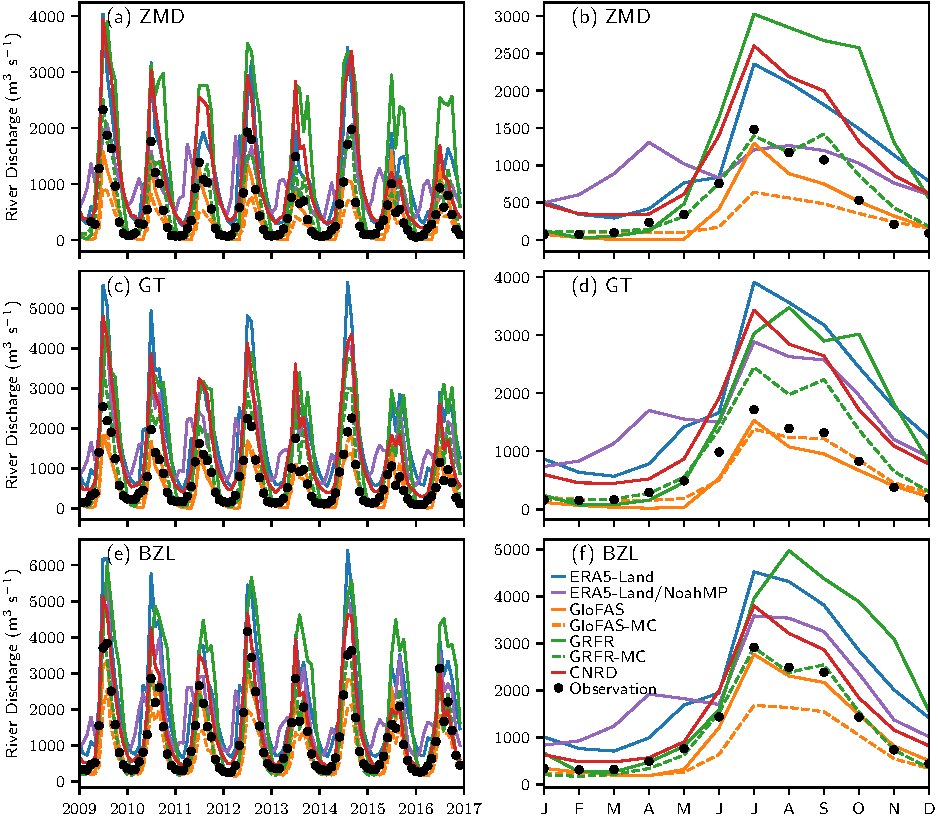
\includegraphics[width=\textwidth]{streamflow_ts.pdf}
  \caption{Same as Figure~\ref{fig:runoff_agg_ts}, but for river discharge.}
  \label{fig:streamflow_ts}
\end{figure}

Figure~\ref{fig:streamflow_dist} presents the river discharge estimates compared with both daily and hourly observations. The aggregated runoff is also displayed for comparison. The difference between the aggregated runoff and the river discharge reveals the impact of river routing. The comparison shows that river routing has a marginal impact in low flow conditions and at the monthly time scale. The impact increases with the flow rate and on shorter time scales. Significant impacts of the river routing are found on the hourly high flow estimations at all gauging stations. This finding suggests the indispensable role of river routing in flood forecasting.

The differences among the examined river discharge estimates are mainly exhibited in high flow conditions. However, these differences do not vary significantly with the time scale of the estimates (i.e., daily or hourly). The GRFR river discharge estimation suspiciously indicates a high probability of discharge at approximately 4000~$\mathrm{m^3\,s^{-1}}$ at all the examined stations, whereas such a high probability is not found in the other estimates including GRFR-MC. This suspicious pattern is another strong evident of inadequate configurations within GRFR's routing process. The GloFAS estimate can well reproduce the observed discharge probability patterns. Our rerouted river discharge using the GloFAS runoff and the Muskingum--Cunge method deviates from the observed pattern of discharge probability. The departure is transferred by the calibration of river discharge from the imprecision in the estimation of river basin areas.

\begin{figure}[ht!]
  \centering
  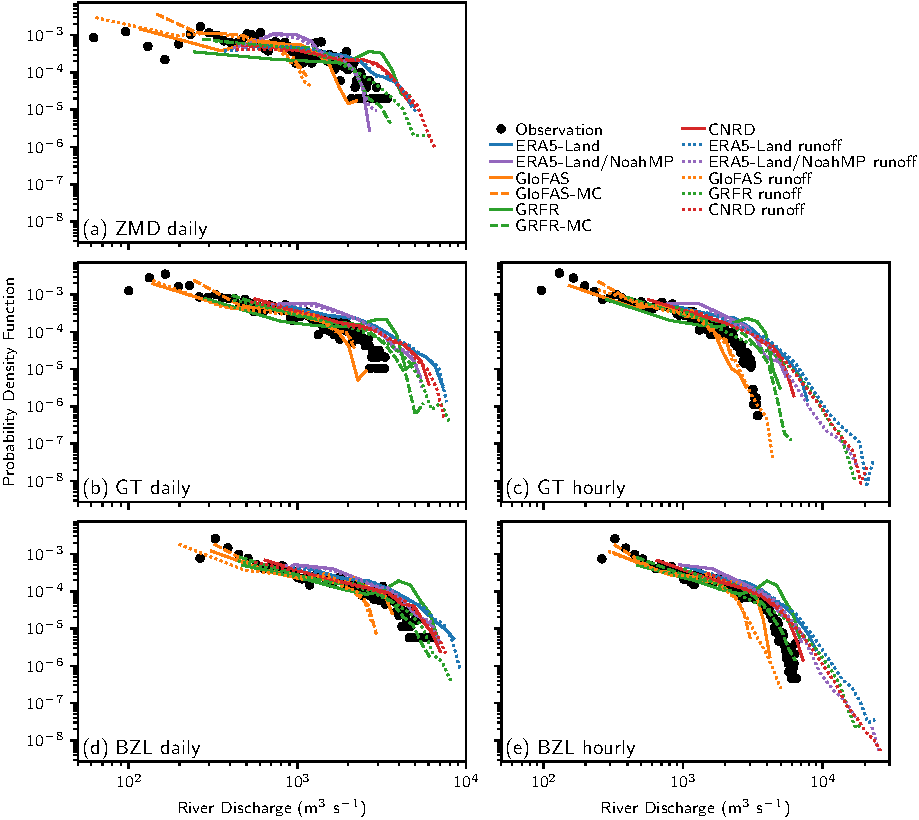
\includegraphics[width=\textwidth]{streamflow_dist_runoff.pdf}
  \caption{Intercomparison of the probability distribution of river discharge and aggregated runoff at the river gauging stations. (a) daily estimates at Zhimenda; (b) hourly estimates at Zhimenda; (c) daily estimates at Gangtuo; (d) hourly estimates at Gangtuo; (e) daily estimates at Benzilan; (f) hourly estimates at Benzilan. Dotted lines denote the aggregated runoff. Solid lines denote the river discharge estimates provided by the examined datasets. Dashed lines denote the river discharge estimates using the runoff and the Muskingum--Cunge routing method. Zhimenda is not shown in the hourly estimates due to the lack of hourly observations.}
  \label{fig:streamflow_dist}
\end{figure}

Figure \ref{fig:streamflow_kge} illustrates the skill scores for the estimation of river discharge across monthly, daily, and hourly temporal scales. At the monthly scale, the river discharge estimation's skill closely mirrors that of the runoff, as depicted in Figure \ref{fig:runoff_kge}. The coincide hints that the primary determinant of river discharge variability within the study area is the runoff estimation, rather than the river routing process. An exception to this pattern is observed with GloFAS, where the divergence in discharge skill scores from those of runoff is likely due to the coarse and imprecise river routing grid employed, as previously discussed.

Among the examined dataset, GloFAS, GloFAS-MC, and GRFR-MC perform the best at all gauging stations and across all time scales. Proper calibration of the land surface model and the hydrological model is essential for accurate river discharge estimation. As revealed in Figure~\ref{fig:streamflow_kge_comp}, the primary reasons for the poor performance of the examined datasets, except for GRFR-MC, are errors in reproducing the observed mean and variability of river discharge. GRFR-MC can effectively reproduce the observed mean and variability of river discharge. The KGE of GRFR-MC's hourly discharge can reach a high score of approximately 0.9 at Benzilan, which again confirms the effectiveness of the characteristics-based calibration method. The deviation of the KGE from 1 for GRFR-MC is mainly attributed to the correlation coefficient, which can be further improved through the calibration of the river routing parameters. The exceptionally high skill of GRFR-MC again confirms the effectiveness of the characteristics-based calibration method.

It is worth to note that the KGE (Figure~\ref{fig:streamflow_kge}) and the relative contribution within the KGE (Figure~\ref{fig:streamflow_kge_comp}) are consistent for both hourly and daily estimates. This consistency suggests that calibration at the daily time scale could potentially be applied to the hourly time scale. The KGE of river discharge is also consistent between daily and monthly estimates for most datasets, with the exception of the high-resolution ERA5-Land/NoahMP estimation. The increase in KGE from the monthly to daily time scale indicates that a more accurate representation of the spatial distribution of runoff and river routing could improve the temporal variations in river discharge estimates, aligning with the concept of the time of concentration \citep{beven2020HESS}. However, these findings are based on a limited number of gauging stations and a limited time period. Further studies are needed to confirm these preliminary observations.

\begin{figure}[ht!]
  \centering
  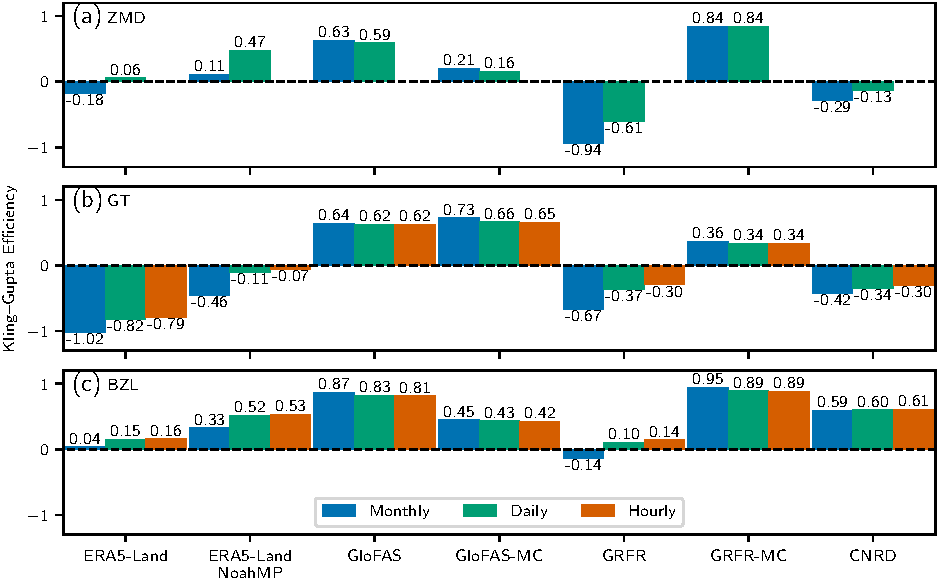
\includegraphics[width=\textwidth]{streamflow_kge.pdf}
  \caption{Kling--Gupta Efficiency of the river discharge estimation. (a) the measures at the Zhimenda station, (b) the measures at the Gangtuo station, and (c) the measures at the Benzilan station.}
  \label{fig:streamflow_kge}
\end{figure}

\begin{figure}[ht!]
  \centering
  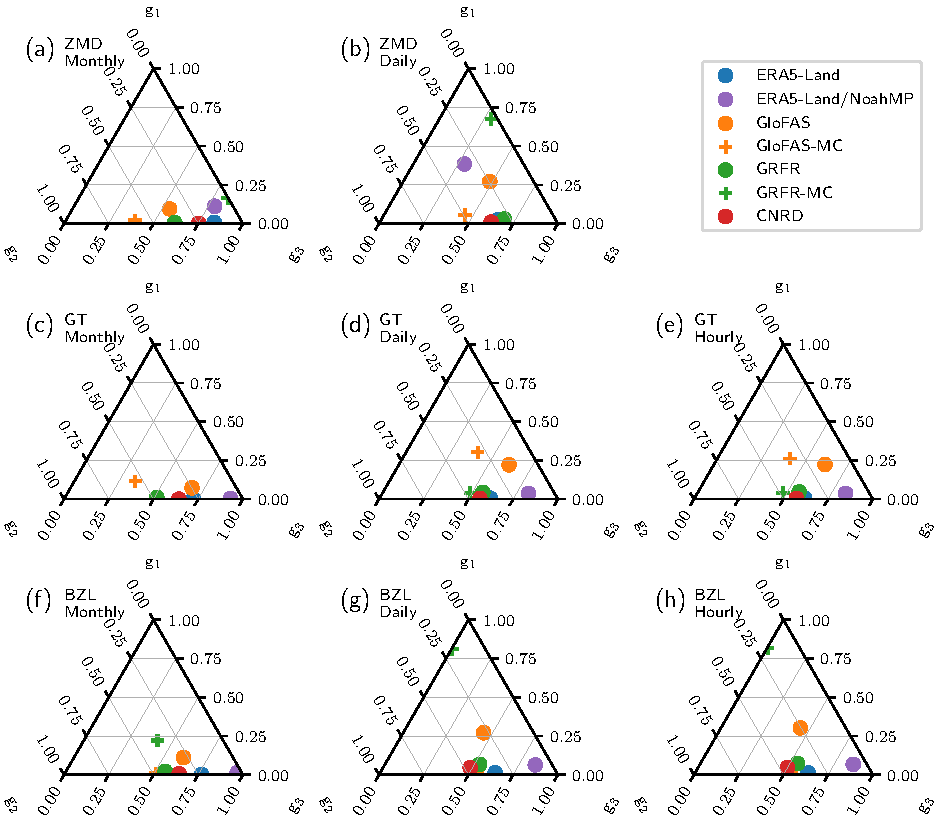
\includegraphics[width=\textwidth]{streamflow_kge_comp.pdf}
  \caption{Ternary plot showing the relative contribution of correlation coefficient ($g_1$), variability ($g_2$), and bias ($g_3$) to the deviation of the Kling--Gupta Efficiency of simulated river discharge from one. The three rows of the plot represent the estimation at Zhimenda, Gangtuo, and Benzilan, respectively. The three columns of the plot represent the results of the monthly, daily, and hourly estimates, respectively.}
  \label{fig:streamflow_kge_comp}
\end{figure}

\section{Conclusions}

This study presents a pilot intercomparison of several publicly available large-domain reanalysis datasets of runoff and river discharge in the Upper Jinsha River basin. The datasets under scrutiny include ERA5-Land, GloFAS, GRFR, and CNRD. To enhance the understanding of the effects of calibration, spatial resolution, and meteorological forcing on runoff estimation, a high-resolution runoff simulation has been incorporated into the comparison. The runoff from the examined datasets is rerouted on a high-resolution river network delineated from the 3-arcsecond MERIT-Hydro dataset. This rerouting aids in identifying the impacts of different river routing models and river network delineations on river discharge estimation. The estimated runoff and river discharge are compared with observations at three gauging stations—Zhimenda, Gangtuo, and Benzilan—spanning monthly, daily, and hourly time scales. The principal findings of this study are as follows:

\begin{itemize}
  \item The examined runoff and river discharge reanalysis datasets display significant discrepancies. When compared with observations, the Kling-Gupta Efficiency of river discharge closely aligns with that of runoff. The primary determinant of river discharge variability within the study area is runoff estimation, rather than the river routing process. The data and models used in runoff estimation need further scrutinization.
  \item Variations in runoff estimates are predominantly attributed to the calibration processes of land surface and hydrological models. Among the datasets, GloFAS and GRFR, which have been calibrated, demonstrate superior performance in runoff estimation. GloFAS and GRFR show similar runoff patterns, despite being driven by different meteorological forcing data. In contrast, the runoff estimates from GloFAS markedly diverge from those of ERA5-Land, even though the meteorological forcing data are similar.
  \item The runoff characteristics-based calibration method shows to be highly effective. GRFR, which employs this method, exhibits the best performance among the examined datasets in terms of runoff estimation. An uncalibrated re-routing using the Muskingum-Cunge method with GRFR runoff can achieve the best performance in estimated river discharge among the examined datasets. However, the river discharge of GRFR exhibits unexpected deterioration, likely due to inadequate configurations in the river routing model.
  \item The river routing process shows its significance during high flow conditions and at time scales shorter than a month. This finding underscores the importance of incorporating a river routing model in flood forecasting. Conversely, the impact of river routing is minimal in low flow conditions and at the monthly time scale. The similarity in monthly aggregated runoff and river discharge estimates allows for an examination of the adequacy of the river routing model and the river network delineation.
  \item A high-resolution river network for flow routing is crucial for concurrent runoff and river discharge estimation. The intercomparison shows a contradiction between GloFAS's high skill in river discharge estimation and a relatively low skill in runoff estimation. The contradiction is likely due to its coarse river routing grid. The coarse grid introduces errors in catchment area estimation, which are then transferred to the runoff estimates during the calibration of river discharge.
  \item High-resolution runoff simulations exhibit distinct runoff characteristics compared to their low-resolution counterparts. While the calibration of high-resolution runoff models can ameliorate these discrepancies, inherent differences in parameter settings between the two resolutions may still result in persistent divergences within other facets of the hydrological cycle.
\end{itemize}

In summary, this study underscores the critical role of model calibration within hydrological modeling and advocates for the integration of high-resolution hydrography data. The results provide significant insights into the enhancement of runoff and streamflow estimation accuracy, which are essential for effective water resource management and the early warning of flood risks in the Upper Jinsha River, and likely in other regions with analogous hydrological attributes.

\section*{Declaration of competing interest}

The authors declare that they have no known competing financial interests or personal relationships that could have appeared to influence the work reported in this paper.

\section*{Data availability}

The MERIT-Hydro dataset was obtained from \url{https://hydro.iis.u-tokyo.ac.jp/~yamadai/MERIT_Hydro/} (accessed on 2024-11-10). The ERA5-Land dataset was obtained from \url{https://cds.climate.copernicus.eu/datasets/reanalysis-era5-land}. The GloFAS v4.0 dataset was obtained from \url{https://ewds.climate.copernicus.eu/datasets/cems-glofas-historical} (accessed on 2024-11-10). The GRFR v1.0 dataset was obtained from \url{https://www.reachhydro.org/home/records/grfr} (accessed on 2024-11-10). The COMIDs used to extract the river discharge from GRFR are 43037713 for Zhimenda, 43046824 for Gangtuo, and 43066085 for Benzilan, respectively. The CNRD v1.0 dataset was obtained from \url{https://doi.org/10.11888/Atmos.tpdc.272864} (accessed on 2024-11-10). The river discharge observations were obtained from the China Three Gorges Corporation; however, the authors do not have permission to share the data.

\section*{Acknowledgements}
This study is supported by China Three Gorges Corporation (contract Z532302035), the National Key Research and Development Program of China (2023YFF0805501), and the Natural Science Foundation of China (grants 42075165 and 42275178). We thank for the technical support of the National Large Scientific Infrastructure ``Earth System Numerical Simulation Facility'' (\url{https://cstr.cn/31134.02.EL}).

\bibliographystyle{elsarticle-harv}
\bibliography{references}

\end{document}
